%% 3-page course report (references on a separate page, not counted). Numbers: % AUTO-GENERATED by R/07_figures_tables.R -- do not edit
\newcommand{\ReEightyFive}{0.89 (0.82 to 0.95)}
\newcommand{\ReEightyThree}{0.74 (0.68 to 0.79)}
\newcommand{\ReFiftyFive}{0.95 (0.86 to 1.02)}
\newcommand{\ReFiftyThree}{0.87 (0.80 to 0.93)}
\newcommand{\ReHundredFive}{0.83 (0.77 to 0.88)}
\newcommand{\ReHundredThree}{0.60 (0.55 to 0.64)}
\newcommand{\ReMedEightyFive}{0.89}
\newcommand{\ReMedEightyThree}{0.74}
\newcommand{\ReMedFiftyFive}{0.95}
\newcommand{\ReMedFiftyThree}{0.87}
\newcommand{\ReMedHundredFive}{0.83}
\newcommand{\ReMedHundredThree}{0.60}
\newcommand{\aIsoFive}{58\%}
\newcommand{\aIsoSeven}{50\%}
\newcommand{\aIsoThree}{70\%}
\newcommand{\avertEightyFive}{22,821 (5,312 to 90,341)}
\newcommand{\avertEightyThree}{27,786 (7,467 to 102,382)}
\newcommand{\avertFiftyFive}{15,595 (3,200 to 64,632)}
\newcommand{\avertFiftyThree}{23,490 (5,527 to 93,061)}
\newcommand{\avertHundredFive}{26,062 (6,700 to 98,336)}
\newcommand{\avertHundredThree}{29,088 (8,364 to 103,935)}
\newcommand{\avertedEightyFive}{22,821}
\newcommand{\avertedEightyThree}{27,786}
\newcommand{\avertedFiftyFive}{15,595}
\newcommand{\avertedFiftyThree}{23,490}
\newcommand{\avertedHundredFive}{26,062}
\newcommand{\avertedHundredThree}{29,088}
\newcommand{\baseCases}{31,089 (9,845 to 107,831)}
\newcommand{\baseCasesMed}{31,089}
\newcommand{\cfrAssumed}{48\%}
\newcommand{\critReEightyFive}{1.13}
\newcommand{\critReEightyThree}{1.36}
\newcommand{\critReFiftyFive}{1.06}
\newcommand{\critReFiftyThree}{1.15}
\newcommand{\critReHundredFive}{1.20}
\newcommand{\critReHundredThree}{1.67}
\newcommand{\crudeCFR}{48\%}
\newcommand{\deathsEightyFive}{11,023}
\newcommand{\deathsEightyThree}{13,421}
\newcommand{\deathsFiftyFive}{7,532}
\newcommand{\deathsFiftyThree}{11,346}
\newcommand{\deathsHundredFive}{12,588}
\newcommand{\deathsHundredThree}{14,050}
\newcommand{\delayHalf}{7}
\newcommand{\delayMean}{8.5}
\newcommand{\delayNinety}{15}
\newcommand{\desolveVersion}{1.40}
\newcommand{\durEightyFive}{24}
\newcommand{\durEightyThree}{9}
\newcommand{\durFiftyFive}{53}
\newcommand{\durFiftyThree}{22}
\newcommand{\durHiEightyFive}{53}
\newcommand{\durHiEightyThree}{14}
\newcommand{\durHiFiftyFive}{$>$60}
\newcommand{\durHiFiftyThree}{49}
\newcommand{\durHiHundredFive}{21}
\newcommand{\durHiHundredThree}{7}
\newcommand{\durHundredFive}{13}
\newcommand{\durHundredThree}{5}
\newcommand{\durLoEightyFive}{14}
\newcommand{\durLoEightyThree}{7}
\newcommand{\durLoFiftyFive}{21}
\newcommand{\durLoFiftyThree}{13}
\newcommand{\durLoHundredFive}{9}
\newcommand{\durLoHundredThree}{4}
\newcommand{\fitAReAfter}{1.04 (0.98 to 1.07)}
\newcommand{\fitAReAfterMed}{1.04}
\newcommand{\fitAReBefore}{1.19 (1.13 to 1.27)}
\newcommand{\fitAReBeforeMed}{1.19}
\newcommand{\fitAacf}{0.27}
\newcommand{\fitAcover}{96\%}
\newcommand{\fitAdAIC}{14.5}
\newcommand{\fitAincEnd}{63 (55 to 71)}
\newcommand{\fitAincEndMed}{63}
\newcommand{\fitApGrow}{0.95}
\newcommand{\fitArAfter}{0.004 ($-$0.001 to 0.006)}
\newcommand{\fitArBefore}{0.017 (0.011 to 0.023)}
\newcommand{\fitAtc}{5 July}
\newcommand{\fitAtcRange}{28 June to 2 August}
\newcommand{\fitBReAfter}{1.00 (0.93 to 1.06)}
\newcommand{\fitBReAfterMed}{1.00}
\newcommand{\fitBReBefore}{1.20 (1.16 to 1.25)}
\newcommand{\fitBReBeforeMed}{1.20}
\newcommand{\fitBacf}{0.01}
\newcommand{\fitBcover}{95\%}
\newcommand{\fitBdAIC}{15.4}
\newcommand{\fitBincEnd}{83 (68 to 100)}
\newcommand{\fitBincEndMed}{83}
\newcommand{\fitBpGrow}{0.56}
\newcommand{\fitBrAfter}{0.000 ($-$0.006 to 0.006)}
\newcommand{\fitBrBefore}{0.018 (0.014 to 0.022)}
\newcommand{\fitBtc}{24 July}
\newcommand{\fitBtcRange}{18 July to 7 August}
\newcommand{\fracIsoBase}{51\%}
\newcommand{\fracIsoEightyFive}{59\%}
\newcommand{\fracIsoEightyThree}{71\%}
\newcommand{\fracIsoFiftyFive}{59\%}
\newcommand{\fracIsoFiftyThree}{71\%}
\newcommand{\fracIsoHundredFive}{59\%}
\newcommand{\fracIsoHundredThree}{71\%}
\newcommand{\meanSep}{86}
\newcommand{\nConfirmed}{7,200}
\newcommand{\nDeaths}{3,475}
\newcommand{\nDraws}{1,000}
\newcommand{\nIntervals}{96}
\newcommand{\nOnsetCases}{4,724}
\newcommand{\nOnsetDays}{105}
\newcommand{\nPRCC}{1,500}
\newcommand{\nRetro}{272}
\newcommand{\nStoch}{500}
\newcommand{\nVarDraws}{300}
\newcommand{\nVariants}{17}
\newcommand{\nVintages}{55}
\newcommand{\nhIncMax}{84}
\newcommand{\nhIncMin}{81}
\newcommand{\nhRMax}{0.0009}
\newcommand{\nhRMin}{$-$0.0005}
\newcommand{\pEndBaseSixty}{0.12}
\newcommand{\pEndBaseTwentyFour}{0.01}
\newcommand{\pEndYearFiveEightyFive}{0.99}
\newcommand{\pEndYearFiveEightyThree}{1.00}
\newcommand{\pEndYearFiveFiftyFive}{0.58}
\newcommand{\pEndYearFiveFiftyThree}{0.99}
\newcommand{\pEndYearFiveHundredFive}{1.00}
\newcommand{\pEndYearFiveHundredThree}{1.00}
\newcommand{\pEndYearOneEightyFive}{0.01}
\newcommand{\pEndYearOneEightyThree}{0.90}
\newcommand{\pEndYearOneFiftyFive}{0.00}
\newcommand{\pEndYearOneFiftyThree}{0.01}
\newcommand{\pEndYearOneHundredFive}{0.33}
\newcommand{\pEndYearOneHundredThree}{1.00}
\newcommand{\pEndYearTwoEightyFive}{0.52}
\newcommand{\pEndYearTwoEightyThree}{1.00}
\newcommand{\pEndYearTwoFiftyFive}{0.05}
\newcommand{\pEndYearTwoFiftyThree}{0.60}
\newcommand{\pEndYearTwoHundredFive}{0.99}
\newcommand{\pEndYearTwoHundredThree}{1.00}
\newcommand{\pReBaseBelow}{0.44}
\newcommand{\pReBelowEightyFive}{1.00}
\newcommand{\pReBelowEightyThree}{1.00}
\newcommand{\pReBelowFiftyFive}{0.94}
\newcommand{\pReBelowFiftyThree}{1.00}
\newcommand{\pReBelowHundredFive}{1.00}
\newcommand{\pReBelowHundredThree}{1.00}
\newcommand{\pctEightyFive}{73 (55 to 84)}
\newcommand{\pctEightyThree}{89 (76 to 95)}
\newcommand{\pctFiftyFive}{50 (33 to 62)}
\newcommand{\pctFiftyThree}{75 (57 to 86)}
\newcommand{\pctHundredFive}{84 (68 to 93)}
\newcommand{\pctHundredThree}{94 (85 to 98)}
\newcommand{\pctMedEightyFive}{73\%}
\newcommand{\pctMedEightyThree}{89\%}
\newcommand{\pctMedFiftyFive}{50\%}
\newcommand{\pctMedFiftyThree}{75\%}
\newcommand{\pctMedHundredFive}{84\%}
\newcommand{\pctMedHundredThree}{94\%}
\newcommand{\popAtRisk}{4,392,200}
\newcommand{\posJun}{22.6}
\newcommand{\posSep}{17.1}
\newcommand{\prccGrowthRate}{0.42}
\newcommand{\prccInfectiousPeriod}{0.10}
\newcommand{\prccIsolationDelay}{0.94}
\newcommand{\prccIsolationEffectiveness}{$-$0.80}
\newcommand{\prccLatentPeriod}{0.27}
\newcommand{\prccStartingIncidence}{0.17}
\newcommand{\rVersion}{4.3.3 (2024-02-29)}
\newcommand{\rYear}{2024}
\newcommand{\shareOnset}{66\%}
\newcommand{\stochBase}{32,114}
\newcommand{\stochEndBase}{0.31}
\newcommand{\stochEndFive}{0.73}
\newcommand{\stochEndThree}{0.86}
\newcommand{\stochFive}{8,904}
\newcommand{\stochRatioMax}{1.09}
\newcommand{\stochRatioMin}{1.00}
\newcommand{\stochRedFive}{72\%}
\newcommand{\stochRedThree}{89\%}
\newcommand{\stochThree}{3,588}
\newcommand{\testsJun}{168}
\newcommand{\testsSep}{494}
\newcommand{\valCumMod}{10,981}
\newcommand{\valCumObs}{10,274}
\newcommand{\valErrLong}{23\%}
\newcommand{\valErrShort}{35\%}
\newcommand{\valInsideLong}{inside}
\newcommand{\valInsideShort}{outside}
\newcommand{\valModLong}{3,781}
\newcommand{\valModLongCI}{3,781 (2,796 to 4,991)}
\newcommand{\valModShort}{1,236}
\newcommand{\valNaiveErrLong}{24\%}
\newcommand{\valObsLong}{3,074}
\newcommand{\valObsShort}{916}
\newcommand{\valPredLongHi}{5,126}
\newcommand{\valPredLongLo}{2,743}
\newcommand{\valRateObsLong}{67}
\newcommand{\valRateObsShort}{61}
\newcommand{\varBaseFourFive}{$-$67 ($-$98 to $-$37)}
\newcommand{\varBaseFourThree}{80 (63 to 90)}
\newcommand{\varCondFive}{83}
\newcommand{\varCondIso}{6\%}
\newcommand{\varCondThree}{93}
\newcommand{\varErlangTenFive}{78}
\newcommand{\varErlangTenThree}{91}
\newcommand{\varErlangThreeFive}{77}
\newcommand{\varFitABase}{51,067}
\newcommand{\varFitAFive}{82}
\newcommand{\varFitAThree}{94}
\newcommand{\varFiveMax}{84}
\newcommand{\varFiveMin}{56}
\newcommand{\varGrowthHiBase}{92,275}
\newcommand{\varGrowthHiFive}{84}
\newcommand{\varGrowthHiThree}{96}
\newcommand{\varGrowthLoBase}{11,750}
\newcommand{\varGrowthLoFive}{56}
\newcommand{\varGrowthLoThree}{77}
\newcommand{\varIncHiFive}{73}
\newcommand{\varIncLoFive}{73}
\newcommand{\varPopFive}{73}
\newcommand{\varRampNinetyFive}{62}
\newcommand{\varRampNinetyThree}{81}
\newcommand{\varRampNinetyUiLo}{40}
\newcommand{\varRampThirtyFive}{69}
\newcommand{\varRampThirtyThree}{86}
\newcommand{\varThreeMax}{96}
\newcommand{\varThreeMin}{77}
 (written by R/07_figures_tables.R)
\documentclass[10pt,a4paper]{article}
\usepackage[T1]{fontenc}\usepackage[utf8]{inputenc}\usepackage{lmodern,microtype}
\usepackage[margin=1.7cm,top=1.5cm,bottom=1.6cm]{geometry}
\usepackage{amsmath,amssymb,booktabs,graphicx,xcolor,caption,enumitem,float,array}
\usepackage[numbers,sort&compress]{natbib}
\usepackage{tikz}\usetikzlibrary{arrows.meta,positioning}
\usepackage[colorlinks,linkcolor=blue!50!black,citecolor=blue!50!black,urlcolor=blue!50!black]{hyperref}
% AUTO-GENERATED by R/07_figures_tables.R -- do not edit
\newcommand{\ReEightyFive}{0.89 (0.82 to 0.95)}
\newcommand{\ReEightyThree}{0.74 (0.68 to 0.79)}
\newcommand{\ReFiftyFive}{0.95 (0.86 to 1.02)}
\newcommand{\ReFiftyThree}{0.87 (0.80 to 0.93)}
\newcommand{\ReHundredFive}{0.83 (0.77 to 0.88)}
\newcommand{\ReHundredThree}{0.60 (0.55 to 0.64)}
\newcommand{\ReMedEightyFive}{0.89}
\newcommand{\ReMedEightyThree}{0.74}
\newcommand{\ReMedFiftyFive}{0.95}
\newcommand{\ReMedFiftyThree}{0.87}
\newcommand{\ReMedHundredFive}{0.83}
\newcommand{\ReMedHundredThree}{0.60}
\newcommand{\aIsoFive}{58\%}
\newcommand{\aIsoSeven}{50\%}
\newcommand{\aIsoThree}{70\%}
\newcommand{\avertEightyFive}{22,821 (5,312 to 90,341)}
\newcommand{\avertEightyThree}{27,786 (7,467 to 102,382)}
\newcommand{\avertFiftyFive}{15,595 (3,200 to 64,632)}
\newcommand{\avertFiftyThree}{23,490 (5,527 to 93,061)}
\newcommand{\avertHundredFive}{26,062 (6,700 to 98,336)}
\newcommand{\avertHundredThree}{29,088 (8,364 to 103,935)}
\newcommand{\avertedEightyFive}{22,821}
\newcommand{\avertedEightyThree}{27,786}
\newcommand{\avertedFiftyFive}{15,595}
\newcommand{\avertedFiftyThree}{23,490}
\newcommand{\avertedHundredFive}{26,062}
\newcommand{\avertedHundredThree}{29,088}
\newcommand{\baseCases}{31,089 (9,845 to 107,831)}
\newcommand{\baseCasesMed}{31,089}
\newcommand{\cfrAssumed}{48\%}
\newcommand{\critReEightyFive}{1.13}
\newcommand{\critReEightyThree}{1.36}
\newcommand{\critReFiftyFive}{1.06}
\newcommand{\critReFiftyThree}{1.15}
\newcommand{\critReHundredFive}{1.20}
\newcommand{\critReHundredThree}{1.67}
\newcommand{\crudeCFR}{48\%}
\newcommand{\deathsEightyFive}{11,023}
\newcommand{\deathsEightyThree}{13,421}
\newcommand{\deathsFiftyFive}{7,532}
\newcommand{\deathsFiftyThree}{11,346}
\newcommand{\deathsHundredFive}{12,588}
\newcommand{\deathsHundredThree}{14,050}
\newcommand{\delayHalf}{7}
\newcommand{\delayMean}{8.5}
\newcommand{\delayNinety}{15}
\newcommand{\desolveVersion}{1.40}
\newcommand{\durEightyFive}{24}
\newcommand{\durEightyThree}{9}
\newcommand{\durFiftyFive}{53}
\newcommand{\durFiftyThree}{22}
\newcommand{\durHiEightyFive}{53}
\newcommand{\durHiEightyThree}{14}
\newcommand{\durHiFiftyFive}{$>$60}
\newcommand{\durHiFiftyThree}{49}
\newcommand{\durHiHundredFive}{21}
\newcommand{\durHiHundredThree}{7}
\newcommand{\durHundredFive}{13}
\newcommand{\durHundredThree}{5}
\newcommand{\durLoEightyFive}{14}
\newcommand{\durLoEightyThree}{7}
\newcommand{\durLoFiftyFive}{21}
\newcommand{\durLoFiftyThree}{13}
\newcommand{\durLoHundredFive}{9}
\newcommand{\durLoHundredThree}{4}
\newcommand{\fitAReAfter}{1.04 (0.98 to 1.07)}
\newcommand{\fitAReAfterMed}{1.04}
\newcommand{\fitAReBefore}{1.19 (1.13 to 1.27)}
\newcommand{\fitAReBeforeMed}{1.19}
\newcommand{\fitAacf}{0.27}
\newcommand{\fitAcover}{96\%}
\newcommand{\fitAdAIC}{14.5}
\newcommand{\fitAincEnd}{63 (55 to 71)}
\newcommand{\fitAincEndMed}{63}
\newcommand{\fitApGrow}{0.95}
\newcommand{\fitArAfter}{0.004 ($-$0.001 to 0.006)}
\newcommand{\fitArBefore}{0.017 (0.011 to 0.023)}
\newcommand{\fitAtc}{5 July}
\newcommand{\fitAtcRange}{28 June to 2 August}
\newcommand{\fitBReAfter}{1.00 (0.93 to 1.06)}
\newcommand{\fitBReAfterMed}{1.00}
\newcommand{\fitBReBefore}{1.20 (1.16 to 1.25)}
\newcommand{\fitBReBeforeMed}{1.20}
\newcommand{\fitBacf}{0.01}
\newcommand{\fitBcover}{95\%}
\newcommand{\fitBdAIC}{15.4}
\newcommand{\fitBincEnd}{83 (68 to 100)}
\newcommand{\fitBincEndMed}{83}
\newcommand{\fitBpGrow}{0.56}
\newcommand{\fitBrAfter}{0.000 ($-$0.006 to 0.006)}
\newcommand{\fitBrBefore}{0.018 (0.014 to 0.022)}
\newcommand{\fitBtc}{24 July}
\newcommand{\fitBtcRange}{18 July to 7 August}
\newcommand{\fracIsoBase}{51\%}
\newcommand{\fracIsoEightyFive}{59\%}
\newcommand{\fracIsoEightyThree}{71\%}
\newcommand{\fracIsoFiftyFive}{59\%}
\newcommand{\fracIsoFiftyThree}{71\%}
\newcommand{\fracIsoHundredFive}{59\%}
\newcommand{\fracIsoHundredThree}{71\%}
\newcommand{\meanSep}{86}
\newcommand{\nConfirmed}{7,200}
\newcommand{\nDeaths}{3,475}
\newcommand{\nDraws}{1,000}
\newcommand{\nIntervals}{96}
\newcommand{\nOnsetCases}{4,724}
\newcommand{\nOnsetDays}{105}
\newcommand{\nPRCC}{1,500}
\newcommand{\nRetro}{272}
\newcommand{\nStoch}{500}
\newcommand{\nVarDraws}{300}
\newcommand{\nVariants}{17}
\newcommand{\nVintages}{55}
\newcommand{\nhIncMax}{84}
\newcommand{\nhIncMin}{81}
\newcommand{\nhRMax}{0.0009}
\newcommand{\nhRMin}{$-$0.0005}
\newcommand{\pEndBaseSixty}{0.12}
\newcommand{\pEndBaseTwentyFour}{0.01}
\newcommand{\pEndYearFiveEightyFive}{0.99}
\newcommand{\pEndYearFiveEightyThree}{1.00}
\newcommand{\pEndYearFiveFiftyFive}{0.58}
\newcommand{\pEndYearFiveFiftyThree}{0.99}
\newcommand{\pEndYearFiveHundredFive}{1.00}
\newcommand{\pEndYearFiveHundredThree}{1.00}
\newcommand{\pEndYearOneEightyFive}{0.01}
\newcommand{\pEndYearOneEightyThree}{0.90}
\newcommand{\pEndYearOneFiftyFive}{0.00}
\newcommand{\pEndYearOneFiftyThree}{0.01}
\newcommand{\pEndYearOneHundredFive}{0.33}
\newcommand{\pEndYearOneHundredThree}{1.00}
\newcommand{\pEndYearTwoEightyFive}{0.52}
\newcommand{\pEndYearTwoEightyThree}{1.00}
\newcommand{\pEndYearTwoFiftyFive}{0.05}
\newcommand{\pEndYearTwoFiftyThree}{0.60}
\newcommand{\pEndYearTwoHundredFive}{0.99}
\newcommand{\pEndYearTwoHundredThree}{1.00}
\newcommand{\pReBaseBelow}{0.44}
\newcommand{\pReBelowEightyFive}{1.00}
\newcommand{\pReBelowEightyThree}{1.00}
\newcommand{\pReBelowFiftyFive}{0.94}
\newcommand{\pReBelowFiftyThree}{1.00}
\newcommand{\pReBelowHundredFive}{1.00}
\newcommand{\pReBelowHundredThree}{1.00}
\newcommand{\pctEightyFive}{73 (55 to 84)}
\newcommand{\pctEightyThree}{89 (76 to 95)}
\newcommand{\pctFiftyFive}{50 (33 to 62)}
\newcommand{\pctFiftyThree}{75 (57 to 86)}
\newcommand{\pctHundredFive}{84 (68 to 93)}
\newcommand{\pctHundredThree}{94 (85 to 98)}
\newcommand{\pctMedEightyFive}{73\%}
\newcommand{\pctMedEightyThree}{89\%}
\newcommand{\pctMedFiftyFive}{50\%}
\newcommand{\pctMedFiftyThree}{75\%}
\newcommand{\pctMedHundredFive}{84\%}
\newcommand{\pctMedHundredThree}{94\%}
\newcommand{\popAtRisk}{4,392,200}
\newcommand{\posJun}{22.6}
\newcommand{\posSep}{17.1}
\newcommand{\prccGrowthRate}{0.42}
\newcommand{\prccInfectiousPeriod}{0.10}
\newcommand{\prccIsolationDelay}{0.94}
\newcommand{\prccIsolationEffectiveness}{$-$0.80}
\newcommand{\prccLatentPeriod}{0.27}
\newcommand{\prccStartingIncidence}{0.17}
\newcommand{\rVersion}{4.3.3 (2024-02-29)}
\newcommand{\rYear}{2024}
\newcommand{\shareOnset}{66\%}
\newcommand{\stochBase}{32,114}
\newcommand{\stochEndBase}{0.31}
\newcommand{\stochEndFive}{0.73}
\newcommand{\stochEndThree}{0.86}
\newcommand{\stochFive}{8,904}
\newcommand{\stochRatioMax}{1.09}
\newcommand{\stochRatioMin}{1.00}
\newcommand{\stochRedFive}{72\%}
\newcommand{\stochRedThree}{89\%}
\newcommand{\stochThree}{3,588}
\newcommand{\testsJun}{168}
\newcommand{\testsSep}{494}
\newcommand{\valCumMod}{10,981}
\newcommand{\valCumObs}{10,274}
\newcommand{\valErrLong}{23\%}
\newcommand{\valErrShort}{35\%}
\newcommand{\valInsideLong}{inside}
\newcommand{\valInsideShort}{outside}
\newcommand{\valModLong}{3,781}
\newcommand{\valModLongCI}{3,781 (2,796 to 4,991)}
\newcommand{\valModShort}{1,236}
\newcommand{\valNaiveErrLong}{24\%}
\newcommand{\valObsLong}{3,074}
\newcommand{\valObsShort}{916}
\newcommand{\valPredLongHi}{5,126}
\newcommand{\valPredLongLo}{2,743}
\newcommand{\valRateObsLong}{67}
\newcommand{\valRateObsShort}{61}
\newcommand{\varBaseFourFive}{$-$67 ($-$98 to $-$37)}
\newcommand{\varBaseFourThree}{80 (63 to 90)}
\newcommand{\varCondFive}{83}
\newcommand{\varCondIso}{6\%}
\newcommand{\varCondThree}{93}
\newcommand{\varErlangTenFive}{78}
\newcommand{\varErlangTenThree}{91}
\newcommand{\varErlangThreeFive}{77}
\newcommand{\varFitABase}{51,067}
\newcommand{\varFitAFive}{82}
\newcommand{\varFitAThree}{94}
\newcommand{\varFiveMax}{84}
\newcommand{\varFiveMin}{56}
\newcommand{\varGrowthHiBase}{92,275}
\newcommand{\varGrowthHiFive}{84}
\newcommand{\varGrowthHiThree}{96}
\newcommand{\varGrowthLoBase}{11,750}
\newcommand{\varGrowthLoFive}{56}
\newcommand{\varGrowthLoThree}{77}
\newcommand{\varIncHiFive}{73}
\newcommand{\varIncLoFive}{73}
\newcommand{\varPopFive}{73}
\newcommand{\varRampNinetyFive}{62}
\newcommand{\varRampNinetyThree}{81}
\newcommand{\varRampNinetyUiLo}{40}
\newcommand{\varRampThirtyFive}{69}
\newcommand{\varRampThirtyThree}{86}
\newcommand{\varThreeMax}{96}
\newcommand{\varThreeMin}{77}

\graphicspath{{../figures/}}
\captionsetup{font=footnotesize,labelfont=bf,skip=2pt}\setlist{nosep,leftmargin=1.2em}
\setlength{\parskip}{2pt}\setlength{\parindent}{0pt}\renewcommand{\arraystretch}{1.05}
\newcommand{\Rt}{R_{\mathrm{e}}}
\pagestyle{plain}
\begin{document}
{\Large\bfseries How fast is fast enough? The onset-to-isolation delay in the 2026 Bundibugyo outbreak, DRC}\\[3pt]
{\small Team TAUS: Oluwafemi Samson Olagbami, Humphrey Rop, Imelda Laetitia Simboro, Jonathan Boakye-Yiadom \;|\; Advisers: Dr James Azam, Andrej Jarynowski \;|\; Preliminary results, November 2026}

\medskip
\noindent\fbox{\parbox{0.975\linewidth}{\small\textbf{Bottom line.} If isolation of symptomatic cases is 80\% effective, cutting the mean delay from onset to isolation from 7 to 5 days would avert about \pctMedEightyFive{} of the next 12 months' cases and from 7 to 3 days about \pctMedEightyThree, turning a plateau ($\Rt\approx\fitBReAfterMed$) into decline. Even at 50\% effectiveness a 3-day delay averts \pctMedFiftyThree. The effect is large because the outbreak sits at the epidemic threshold, and it reverses if the true current delay is already under 5 days, so the delay must be measured.}}

\subsection*{Question and approach}
By 12 September 2026 the DRC had \nConfirmed{} confirmed cases and a modelled incidence of about \fitBincEndMed{} new cases per day. We asked how many cases would be prevented, and how much sooner transmission would end, if the mean delay from symptom onset to isolation fell from 7 to 5 or 3 days, with isolation that is 50\%, 80\% or 100\% effective (reducing transmission of isolated cases by that fraction). We used a deterministic susceptible--exposed--infectious--isolated--removed (SEIQR) model (Fig.~\ref{fig:model}) with isolation rate $\tau=1/\text{delay}$; isolated people transmit at $1-\epsilon$ of the rate of others, so
$\Rt=(\beta/\gamma)\{1-\epsilon\,\tau/(\tau+\gamma)\}$ (details in the manuscript appendix). The model was fitted by maximum likelihood to confirmed cases by report date up to 12 September \citep{bvdoutbreaksize2026}, allowing one change in transmission (cross-checked against the onset curve corrected for reporting delay). It fitted well (95\% predictive coverage \fitBcover). Transmission grew ($\Rt$ \fitBReBeforeMed) until about \fitBtc{} and has since plateaued ($\Rt$ \fitBReAfter).

\begin{figure}[H]\centering
\begin{tikzpicture}[node distance=1.25cm,>=Stealth,box/.style={draw,minimum size=0.6cm,inner sep=2pt},every node/.style={font=\footnotesize}]
\node[box](S){S};\node[box,right=of S](E){E};\node[box,right=of E,draw=red!70!black,thick](I){I};\node[box,right=of I](R){R};\node[box,above=0.7cm of I,draw=red!70!black,thick](Q){Q};
\draw[->](S)--node[above]{$\lambda$}(E);\draw[->](E)--node[above]{$\sigma$}(I);\draw[->](I)--node[above]{$\gamma$}(R);\draw[->](I)--node[left]{$\tau=1/\text{delay}$}(Q);\draw[->](Q)-|node[above,pos=0.2]{$\gamma$}(R);
\node[right=0.8cm of R,align=left]{$\lambda=\beta[I+(1-\epsilon)Q]/N$; $\epsilon$ = isolation effectiveness};
\end{tikzpicture}\caption{Model structure; the intervention is the flow $I\to Q$.}\label{fig:model}\end{figure}

\subsection*{Scenarios and uncertainty}
Nine scenarios (delay 7, 5, 3 days $\times$ $\epsilon$ 50, 80, 100\%) start on 12 September 2026. Each of \nDraws{} paired draws combines the fitted growth rate and incidence with latent (mean 6.3 d, range 4.0--10.1) and infectious periods (mean 7 d, range 5--10) drawn from triangular distributions \citep{ebengo2026,chowell2014}; transmission is calibrated so the 7-day baseline reproduces the fitted growth, and only the delay changes between scenarios. Outcomes: cumulative symptomatic cases over 12 months, cases averted versus the 7-day delay, and months until fewer than one exposed or infectious person remains. We also ran a stochastic version (\nStoch{} replicates), partial-rank-correlation and \nVariants{} structural sensitivity analyses, and an out-of-sample forecast check. All code is in R; the repository regenerates every number and figure.

\subsection*{Results}
\begin{table}[H]\centering\scriptsize\caption{Results (median and 95\% uncertainty interval, \nDraws{} paired draws; $^\dagger$ cases averted $\times$ \cfrAssumed, illustrative).}
\resizebox{\textwidth}{!}{\begin{tabular}{@{}rrcrrrrr@{}}
\toprule
Isolation & Delay & $R_e$ & Cases in 12 months & Cases averted (\%) & Deaths averted$^\dagger$ & Months to end & P(ended $\le$24 mo) \\
effectiveness & (days) & median (95\% UI) & median (95\% UI) & median (95\% UI) & median & median (95\% UI) &  \\
\midrule
50\% & 7 & 1.00 (0.92--1.08) & 31,201 (9,854--109,025) & -- & -- & $>$60 & 0.01 \\
 & 5 & 0.95 (0.86--1.02) & 15,405 (6,232--44,057) & 50 (33--62) & 7,532 & 53 (21 to $>$60) & 0.05 \\
 & 3 & 0.87 (0.80--0.93) & 7,695 (4,033--16,443) & 75 (57--86) & 11,346 & 22 (13 to 49) & 0.60 \\
\midrule
80\% & 7 & 1.00 (0.92--1.07) & 31,089 (9,845--107,831) & -- & -- & $>$60 & 0.01 \\
 & 5 & 0.89 (0.82--0.95) & 8,212 (4,127--18,244) & 73 (55--84) & 11,023 & 24 (14 to 53) & 0.52 \\
 & 3 & 0.74 (0.68--0.79) & 3,313 (2,133--5,309) & 89 (76--95) & 13,421 & 9 (7 to 14) & 1.00 \\
\midrule
100\% & 7 & 1.00 (0.93--1.06) & 30,961 (9,833--106,530) & -- & -- & $>$60 & 0.01 \\
 & 5 & 0.83 (0.77--0.88) & 4,807 (2,779--8,746) & 84 (68--93) & 12,588 & 13 (9 to 21) & 0.99 \\
 & 3 & 0.60 (0.55--0.64) & 1,817 (1,234--2,728) & 94 (85--98) & 14,050 & 5 (4 to 7) & 1.00 \\
\bottomrule
\end{tabular}
}\end{table}
With a 7-day delay the model projects \baseCases{} cases over 12 months and transmission that persists beyond five years. At 80\% effectiveness a 5-day delay lowers $\Rt$ to \ReMedEightyFive{} and a 3-day delay to \ReMedEightyThree, with transmission ending after a median of \durEightyFive{} and \durEightyThree{} months. At 50\% effectiveness the corresponding times are \durFiftyFive{} and \durFiftyThree{} months; at 100\% they are \durHundredFive{} and \durHundredThree{} months. Returns diminish: the first two days saved (7 to 5) avert more than the next two.

\begin{figure}[H]\centering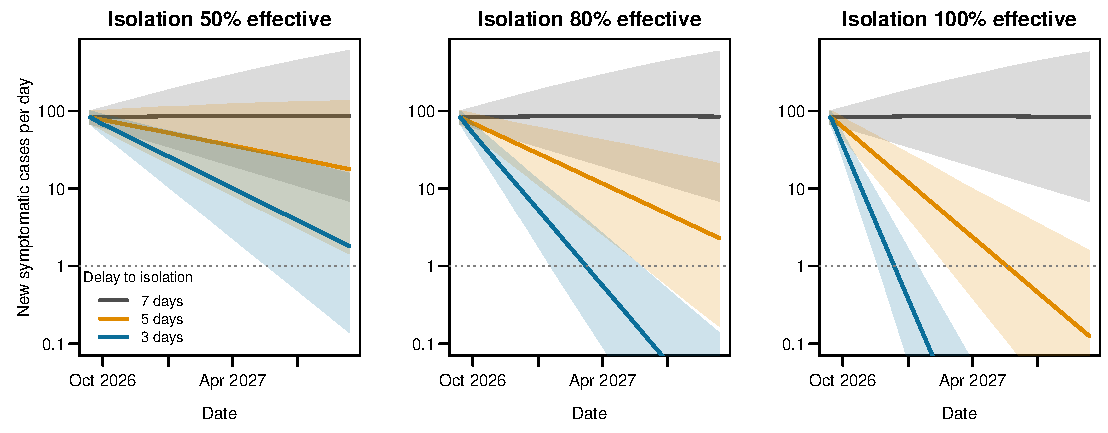
\includegraphics[width=0.97\textwidth]{fig3_trajectories.pdf}\captionof{figure}{Projected new symptomatic cases per day (median and 95\% UI, log scale) from 12 September 2026.}\end{figure}
\vspace{-6pt}
\begin{figure}[H]\centering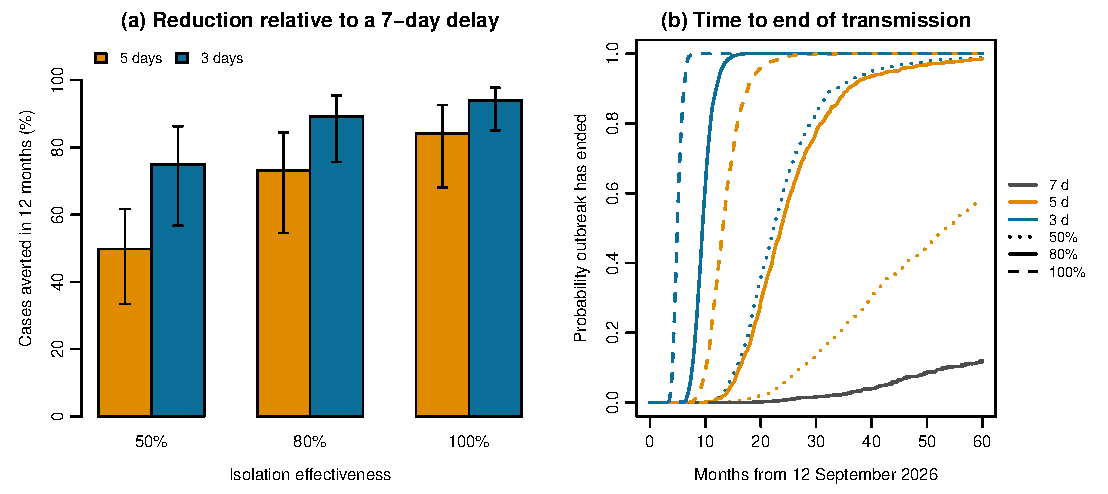
\includegraphics[width=0.97\textwidth]{fig4_averted_duration.pdf}\captionof{figure}{(a) Percent of 12-month cases averted relative to a 7-day delay. (b) Probability transmission has ended, by months.}\end{figure}

\subsection*{How robust is this?}
The stochastic model gave the same medians (ratio \stochRatioMin--\stochRatioMax). The isolation delay (partial rank correlation \prccIsolationDelay) and effectiveness (\prccIsolationEffectiveness) dominate the uncertainty, followed by baseline growth (\prccGrowthRate). Across assumptions (natural history, Erlang-distributed delays, delay defined among isolated cases, 90-day roll-out) the 5-day benefit stayed between \varFiveMin{} and \varFiveMax\% and the 3-day benefit between \varThreeMin{} and \varThreeMax\%. \textbf{The exception is the baseline delay:} if the true current delay were 4.6 days, a ``5-day'' target would increase cases (percentage averted: \varBaseFourFive). A forecast using data to 12 September overestimated the next 46 days of cases by \valErrLong, so absolute counts should be read as conditional on the plateau.

\subsection*{Decision relevance and limits}
Shortening the delay (community alert networks, decentralised sampling, rapid results, nearby isolation capacity) is worth the most when isolation is also effective; a quick delay with poor isolation helps less. Percent reductions apply while the outbreak is near $\Rt\approx1$; at higher $\Rt$ a 3-day delay alone suffices only if baseline $\Rt\le\critReEightyThree$ (80\% effectiveness). Limits: the 7-day baseline comes from the project brief and is not confirmed; isolation effectiveness is assumed, not estimated; infectiousness is constant and contact tracing, funerals and spatial structure are omitted; national data are treated as homogeneous. Code and data: repository README (URL to be added).

\newpage{\footnotesize\bibliographystyle{unsrtnat}\bibliography{../manuscript/references}}
\end{document}
